
\documentclass{article}
\usepackage[spanish]{babel} %Definir idioma español
\usepackage[utf8]{inputenc} %Codificacion utf-8
\usepackage{amssymb, amsmath, amsbsy, wasysym}
\usepackage{multirow} % para tablas
\usepackage{graphicx}
\usepackage[ruled, vlined, spanish, linesnumbered]{algorithm2e} %Para escribir algoritmos
\title{Tarea 1\\Inteligencia artificial}
\author{Emmanuel Peto Gutiérrez}
\begin{document}
\maketitle

\section*{Análisis del algoritmo de búsqueda voraz}

\begin{itemize}
\item \textbf{¿Es completo?}

Si se marcan los nodos visitados sí es completo. En otro caso no lo es, y se mostrará con el siguiente ejemplo. Se tiene la siguiente gráfica con 7 nodos y una tabla con la distancia en línea recta desde cualquier nodo hacia $F$.

\begin{centering}
\includegraphics[scale=0.3]{grafica1}
\hspace{5mm}
\begin{tabular}{|c|c|}
\hline
\textbf{Nodo} & \textbf{Distancia hacia F}\\ \hline
A & 40m \\ \hline
E & 48m \\ \hline
G & 57m \\ \hline
B & 72m \\ \hline
C & 120m \\ \hline
D & 122m\\ \hline
F & 0m \\ \hline
\end{tabular}
\end{centering}

Se empieza la búsqueda en $B$ y el nodo meta es $F$. El vecino de $B$ más cercano a $F$ es $A$, pues su distancia es 40m. Después, desde $A$ la búsqueda debe continuar al nodo vecino de $A$ cuya distancia sea la menor hacia $F$; pero este nodo es $B$, pues es su único vecino. Desde $B$ se mueve otra vez a $A$ y así sucesivamente en un loop infinito. Como se observa en este caso el algoritmo no termina, y por lo tanto es incompleto.

\item \textbf{¿Es óptimo?}

No es óptimo y se pondrá el ejemplo de Rumania. Para ir de Arad a Bucharest usando este algoritmo se procede de la siguiente forma: Arad $\rightarrow$ Sibiu $\rightarrow$ Fagaras $\rightarrow$ Bucharest y el costo del camino es 450. Sin embargo, existe otro camino cuyo costo es 418: Arad $\rightarrow$ Sibiu $\rightarrow$ Rimnicu Vilcea $\rightarrow$ Pitesti $\rightarrow$ Bucharest.

\item \textbf{Complejidad en tiempo}

Debido a que la búsqueda voraz procede en profundidad, la complejidad en tiempo es la misma que en búsqueda en profundidad. Si $d$ es la profundidad máxima del árbol y $b$ es el número máximo de hijos que tiene un nodo, entonces la complejidad en tiempo es $O(b^d)$ en el peor caso.

\item \textbf{Complejidad en espacio}

La complejidad en espacio es la misma que en la búsqueda en profundidad: $O(bd)$.

\end{itemize}

\end{document}

